\documentclass[a4paper, 14pt]{extarticle}
\usepackage[english,russian]{babel}
\usepackage[T1]{fontenc}
\usepackage[utf8]{inputenc}
\usepackage{fontspec}
\usepackage{indentfirst}
\usepackage{enumitem}
\usepackage{graphicx}
\usepackage[
  left=30mm,
  right=10mm,
  top=20mm,
  bottom=20mm
]{geometry}
\usepackage{parskip}
\usepackage{titlesec}
\usepackage{xurl}
\usepackage{hyperref}
\usepackage{float}
\usepackage[
  figurename=Рисунок,
  labelsep=endash,
  justification=centering
]{caption}
\usepackage[outputdir=build, newfloat]{minted}
\usepackage{chngcntr}

\selectlanguage{russian}

\hypersetup{
  colorlinks=true,
  linkcolor=black,
  filecolor=blue,
  urlcolor=blue,
}

\renewcommand*{\labelitemi}{---}
\setmainfont{Times New Roman}
\setmonofont{JetBrains Mono}[
  SizeFeatures={Size=11},
]

\newenvironment{code}{\captionsetup{type=figure}}{}
\BeforeBeginEnvironment{code}{\bigskip}
\AfterEndEnvironment{code}{\bigskip}

\setminted{
  fontsize=\footnotesize,
}

\setlength{\parskip}{6pt}

\setlength{\parindent}{1.25cm}
\setlist[itemize]{itemsep=0em,topsep=0em,parsep=0em,partopsep=0em,leftmargin=2.0cm,wide}
\setlist[enumerate]{itemsep=0em,topsep=0em,parsep=0em,partopsep=0em,leftmargin=2.0cm,wide}

\renewcommand{\thesection}{\indent\arabic{section}.}
\renewcommand{\thesubsection}{\indent\thesection\arabic{subsection}.}
\renewcommand{\thesubsubsection}{\indent\thesubsection\arabic{subsubsection}.}

\titleformat{\section}{\normalfont\bfseries}{\thesection}{0.5em}{}
\titleformat{\subsection}{\normalfont\bfseries}{\thesubsection}{0.5em}{}
\titleformat{\subsubsection}{\normalfont\bfseries}{\thesubsubsection}{0.5em}{}

\titleformat*{\section}{\normalfont\bfseries}
\titleformat*{\subsection}{\normalfont\bfseries}
\titleformat*{\subsubsection}{\normalfont\bfseries}

\titlespacing{\section}{\parindent}{\parskip}{\parskip}
\titlespacing{\subsection}{\parindent}{\parskip}{\parskip}
\titlespacing{\subsubsection}{\parindent}{\parskip}{\parskip}

\begin{document}

\begin{titlepage}
  \vspace{0pt plus2fill}
  \noindent

  \vspace{0pt plus6fill}
  \begin{center}
    {
    \bfseries
    Министерство науки и высшего образования Российской Федерации
    {
    \scriptsize
    ФЕДЕРАЛЬНОЕ ГОСУДАРСТВЕННОЕ АВТОНОМНОЕ ОБРАЗОВАТЕЛЬНОЕ УЧРЕЖДЕНИЕ ВЫСШЕГО
    ОБРАЗОВАНИЯ
    }
    «Национальный исследовательский университет ИТМО»

    (Университет ИТМО)

    \begin{minipage}[t]{0.42\textwidth}
      \vspace*{0pt}
      \begin{flushright}
        Факультет

        Образовательная программа
      \end{flushright}
    \end{minipage}
    \begin{minipage}[t]{0.57\textwidth}
      \vspace*{0pt}
      \begin{flushright}
        Инфокоммуникационных технологий

        11.03.02 Программирование в инфокоммуникационных системах
      \end{flushright}
    \end{minipage}
    }

    \vspace{0pt plus5fill}

    \LARGE{
      ОТЧЕТ

      по лабораторной работе 8

      по дисциплине \textbf{<<Разработка баз данных>>}
    }
  \end{center}

  \vspace{0pt plus4fill}
  \begin{flushright}
    Выполнил: \textbf{студент группы K33211 Швалов Д. А.}

    Проверил: \textbf{ст. преподаватель Осетрова И.С.}
  \end{flushright}

  \vspace{0pt plus8fill}
  \begin{center}
    Санкт-Петербург

    2024
  \end{center}
\end{titlepage}

\setcounter{page}{2}

\linespread{1.5}
\renewcommand{\baselinestretch}{1.5}

\section*{
  \large{Лабораторная работа №8 <<Управление транзакциями и блокировками>>}
 }

\section{Цель работы}

Управление транзакциями и блокировками.

\section{Задачи, решаемые при выполнении работы}

\begin{enumerate}[leftmargin=*]
  \item Определение транзакции.
  \item Поиск и обнаружение блокирования.
  \item Уровни изоляции.
\end{enumerate}

\section{Объект исследования}

Управление транзакциями и блокировками в СУБД
\foreignlanguage{english}{Microsoft SQL Server} с помощью
\foreignlanguage{english}{Microsoft SQL Server Management Studio (SSMS)}.

\section{Исходные данные}

\begin{itemize}
  \item методические указания к лабораторной работе;
  \item СУБД Microsoft SQL Server;
  \item Microsoft SQL Server Management Studio;
  \item база данных ApressFinancial.
\end{itemize}

\section{Выполнение работы}

\subsection{Первая задача}

\subsubsection{Инструкция COMMIT TRAN}

На рисунке \ref{fig:task-1-1} представлен запрос, в котором транзакция
создается, а затем завершается с помощью инструкции
<<\foreignlanguage{english}{COMMIT TRAN}>>. Как видно на рисунке
\ref{fig:task-1-2}, после выполнения запроса изменения, произведенные в
транзакции, были сохранены в базе данных.

\begin{figure}[H]
  \centering
  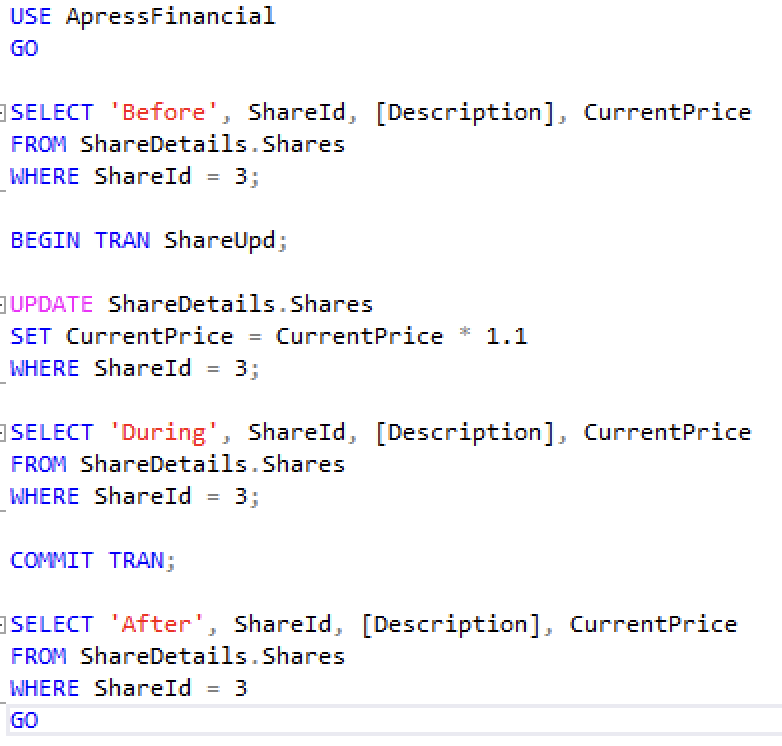
\includegraphics[width=0.8\textwidth]{images/task-1/1.png}
  \caption{
    Завершение транзакции с помощью <<\foreignlanguage{english}{COMMIT TRAN}>>
  }
  \label{fig:task-1-1}
\end{figure}

\begin{figure}[H]
  \centering
  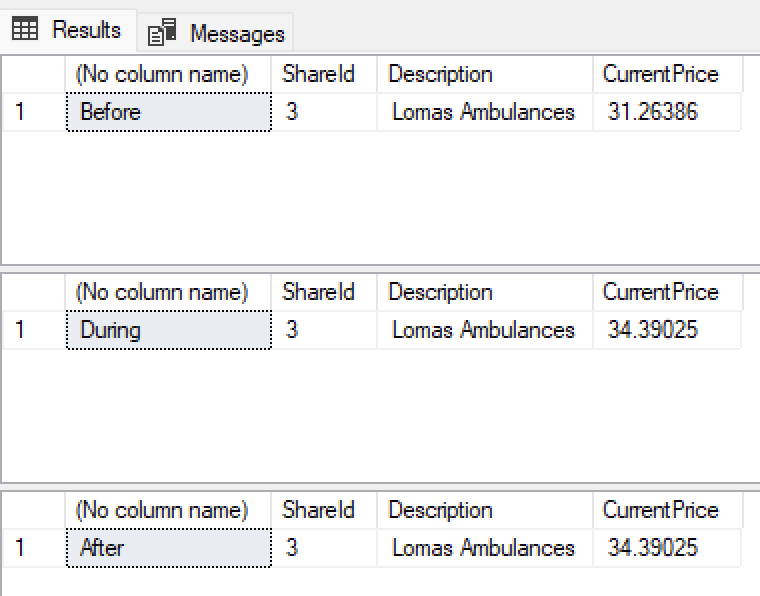
\includegraphics[width=0.7\textwidth]{images/task-1/2.png}
  \caption{Результат выполнения запроса}
  \label{fig:task-1-2}
\end{figure}

\subsubsection{Инструкция ROLLBACK TRAN}

На рисунке \ref{fig:task-1-3} приведен запрос, в котором транзакция завершается
уже с помощью инструкции <<\foreignlanguage{english}{ROLLBACK TRAN}>>. В этом
случае, как видно на рисунке \ref{fig:task-1-4}, изменения не были сохранены в
базе данных.

\begin{figure}[H]
  \centering
  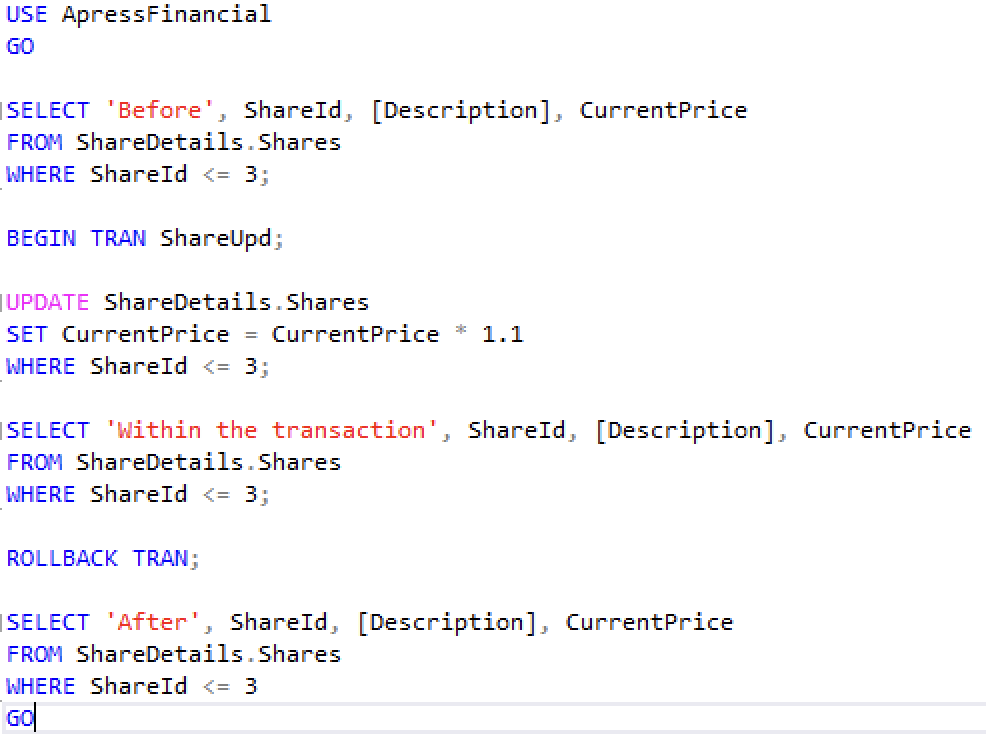
\includegraphics[width=0.8\textwidth]{images/task-1/3.png}
  \caption{
    Завершение транзакции с помощью <<\foreignlanguage{english}{ROLLBACK TRAN}>>
  }
  \label{fig:task-1-3}
\end{figure}

\begin{figure}[H]
  \centering
  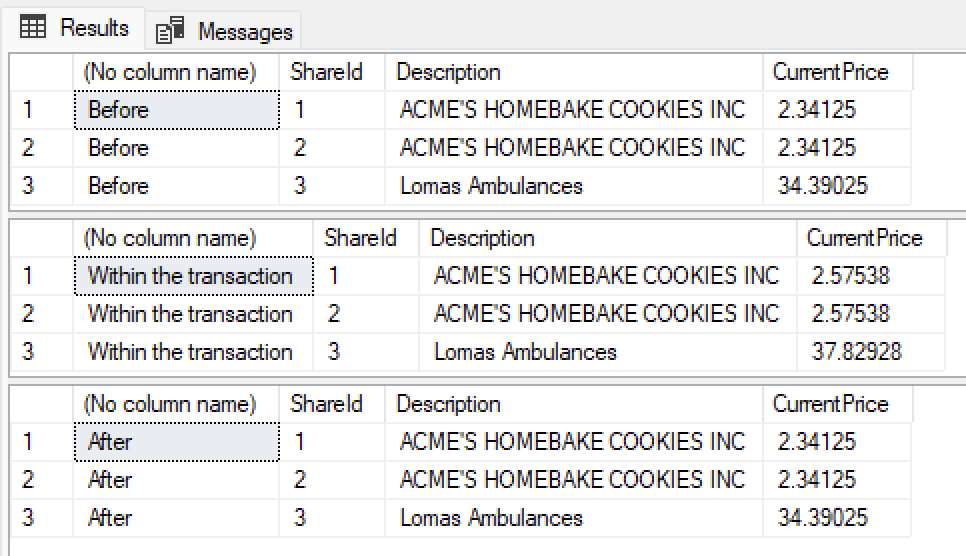
\includegraphics[width=0.7\textwidth]{images/task-1/4.png}
  \caption{Результат выполнения запроса}
  \label{fig:task-1-4}
\end{figure}

\subsubsection{Вложенные транзакции}

На рисунке \ref{fig:task-1-5} приведен запрос, который работает со вложенными
транзакциями. В нем создается две транзакции, при этом вторая находится внутри
первой. Как видно на рисунке \ref{fig:task-1-6}, количество выполняемых
транзакций, с началом каждой транзакции, увеличивается. А при завершении
транзакций это количество уменьшается.

\begin{figure}[H]
  \centering
  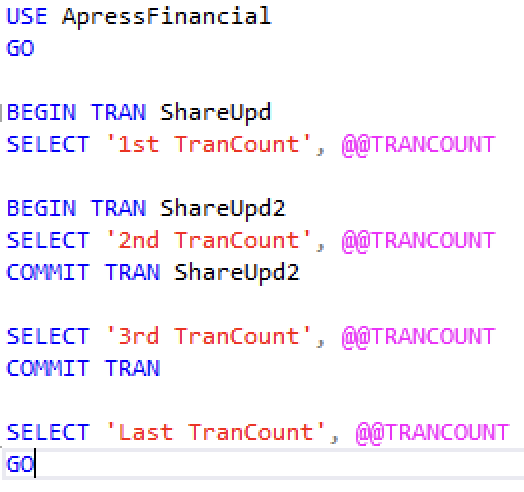
\includegraphics[width=0.5\textwidth]{images/task-1/5.png}
  \caption{Запрос с вложенными транзакциями}
  \label{fig:task-1-5}
\end{figure}

\begin{figure}[H]
  \centering
  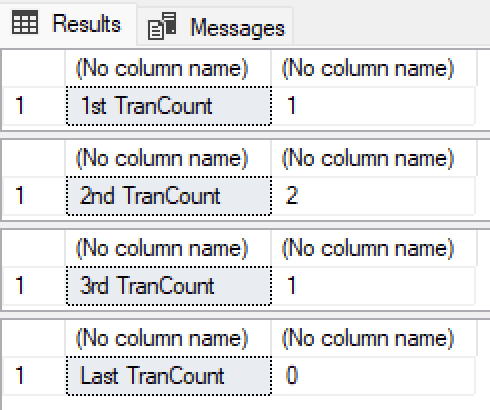
\includegraphics[width=0.6\textwidth]{images/task-1/6.png}
  \caption{Результат выполнения запроса}
  \label{fig:task-1-6}
\end{figure}

\subsection{Вторая задача}

\subsubsection{Создание тестовой базы данных}

С помощью кода из файла
<<\foreignlanguage{english}{SQLQuery\_CREATE\_DB\_exmp\_block.sql}>> был создана
тестовая база данных <<\foreignlanguage{english}{test\_block}>>. После
выполнения кода новая база данных появилась в интерфейсе SSMS (рисунок
\ref{fig:task-2-1}).

\begin{figure}[H]
  \centering
  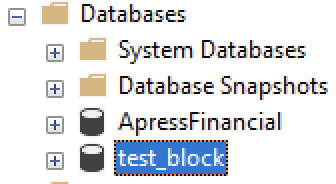
\includegraphics[width=0.4\textwidth]{images/task-2/1.png}
  \caption{Созданная база данных}
  \label{fig:task-2-1}
\end{figure}

\subsubsection{Поиск и обнаружение блокирования}

Для выполнения данного задания были открыты три отдельных окна запросов в SSMS.
В первом окне был введен и выполнен запрос, показанный на рисунке
\ref{fig:task-2-2}. В нем изменяется цена товара с идентификатором 2 внутри
транзакции. При этом транзакция остается открытой. Как видно на рисунке
\ref{fig:task-2-3}, сделанные изменения были применены внутри транзакции.

\begin{figure}[H]
  \centering
  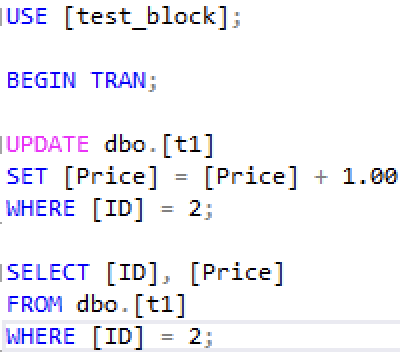
\includegraphics[width=0.5\textwidth]{images/task-2/2.png}
  \caption{Запрос с изменением внутри открытой транзакции}
  \label{fig:task-2-2}
\end{figure}

\begin{figure}[H]
  \centering
  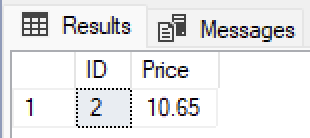
\includegraphics[width=0.4\textwidth]{images/task-2/3.png}
  \caption{Результат выполнения запроса}
  \label{fig:task-2-3}
\end{figure}

Затем во втором окне был выполнен запрос, показанный на рисунке
\ref{fig:task-2-4}. В нем происходит попытка обратиться к строке, которая
заблокирована транзакцией. Поэтому данный запрос не выполнился сразу, а был
поставлен в ожидание.

\begin{figure}[H]
  \centering
  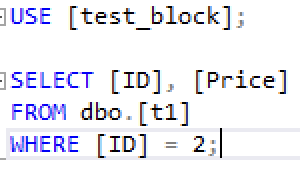
\includegraphics[width=0.4\textwidth]{images/task-2/4.png}
  \caption{Запрос к заблокированной строке таблицы}
  \label{fig:task-2-4}
\end{figure}

В третьем окне был выполнен запрос, показанный на рисунке \ref{fig:task-2-5}. С
его помощью была получена информация о сеансах и заблокированных строках. Как
видно на рисунке \ref{fig:task-2-6}, сеансы с идентификаторами 52 и 69 пытаются
получить доступ к одной и той же строке.

\begin{figure}[H]
  \centering
  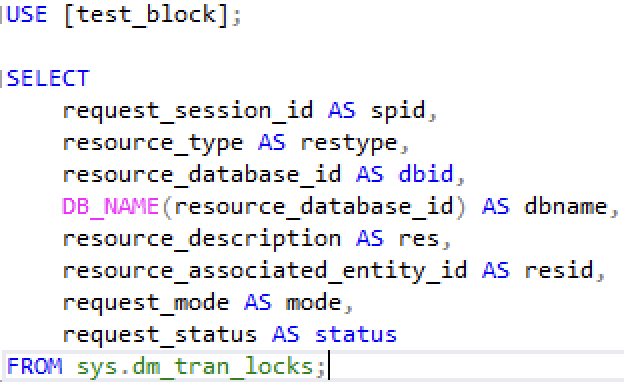
\includegraphics[width=0.7\textwidth]{images/task-2/5.png}
  \caption{Запрос для получения информации о сеансах}
  \label{fig:task-2-5}
\end{figure}

\begin{figure}[H]
  \centering
  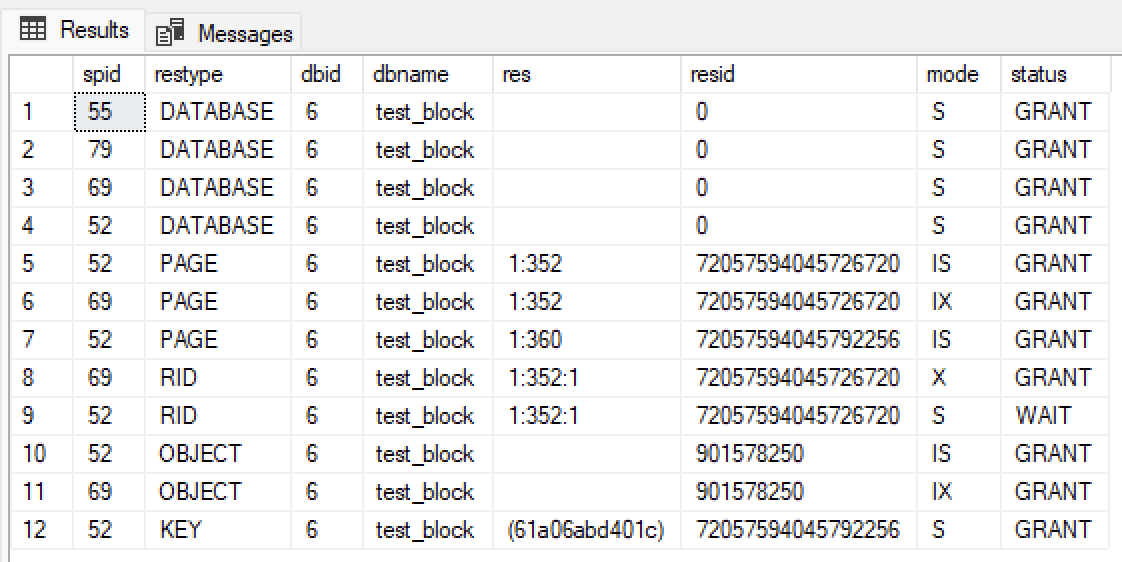
\includegraphics[width=0.8\textwidth]{images/task-2/6.png}
  \caption{Результат выполнения запроса}
  \label{fig:task-2-6}
\end{figure}

С помощью запроса, показанного на рисунке \ref{fig:task-2-7}, для данных сеансов
была получена информация о последних подключениях. Результат выполнения запроса
представлен на рисунке \ref{fig:task-2-8}.

\begin{figure}[H]
  \centering
  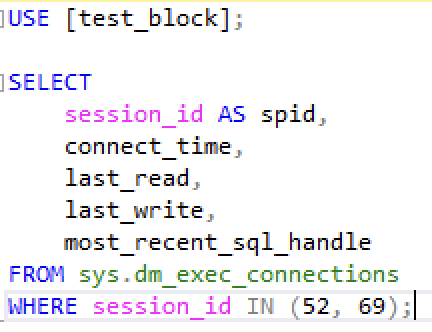
\includegraphics[width=0.5\textwidth]{images/task-2/7.png}
  \caption{Запрос для получения информации о подключениях}
  \label{fig:task-2-7}
\end{figure}

\begin{figure}[H]
  \centering
  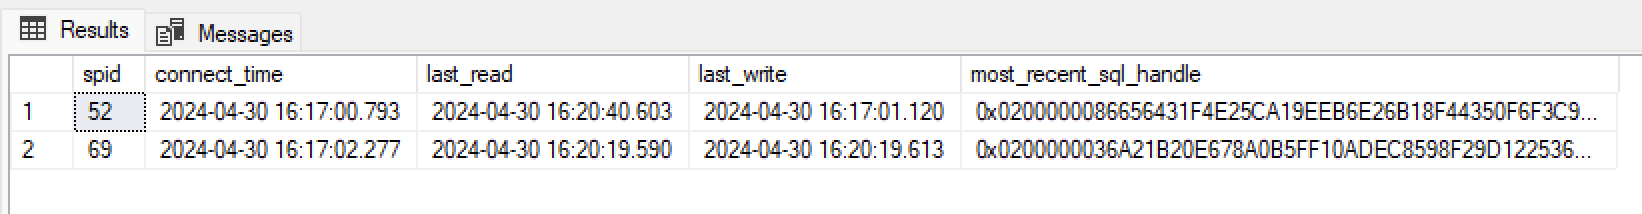
\includegraphics[width=\textwidth]{images/task-2/8.png}
  \caption{Результат выполнения запроса}
  \label{fig:task-2-8}
\end{figure}

С помощью запроса, приведенном на рисунке \ref{fig:task-2-9} были получены
текстовые представления последних запросов для данных сеансов. На рисунке
\ref{fig:task-2-10} показан результат выполнения данного запроса. Данные запросы
совпадают с теми, что были введены в интерфейсе SSMS.

\begin{figure}[H]
  \centering
  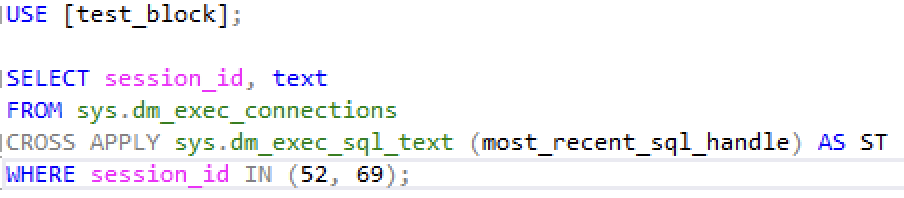
\includegraphics[width=0.9\textwidth]{images/task-2/9.png}
  \caption{Запрос для получения текстового представления запросов сеансов}
  \label{fig:task-2-9}
\end{figure}

\begin{figure}[H]
  \centering
  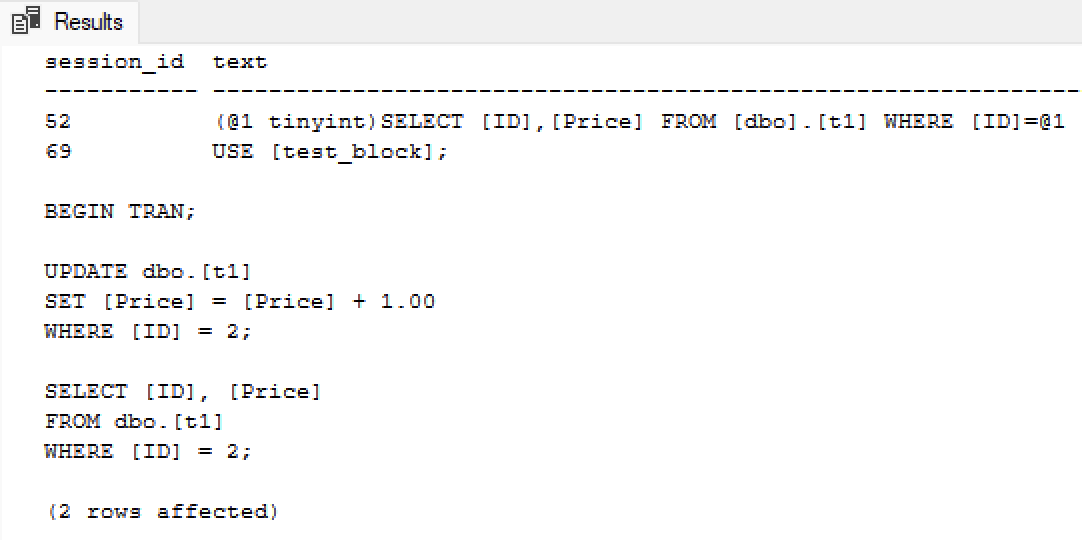
\includegraphics[width=\textwidth]{images/task-2/10.png}
  \caption{Результат выполнения запроса}
  \label{fig:task-2-10}
\end{figure}

На рисунке \ref{fig:task-2-11} представлен запрос, с помощью которого можно
получить идентификаторы заблокированных сеансов. На рисунке \ref{fig:task-2-12}
видно, что идентификаторы сеансов совпадают с теми, что были получены ранее.

\begin{figure}[H]
  \centering
  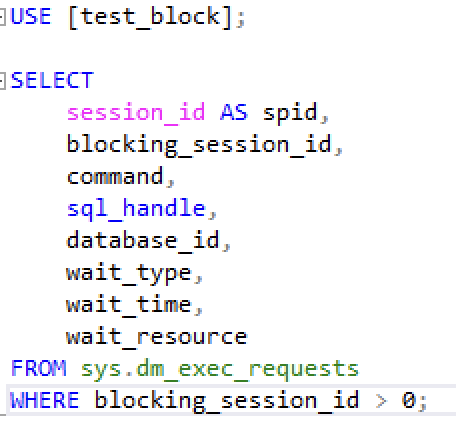
\includegraphics[width=0.5\textwidth]{images/task-2/11.png}
  \caption{Запрос для получения заблокированных сеансов}
  \label{fig:task-2-11}
\end{figure}

\begin{figure}[H]
  \centering
  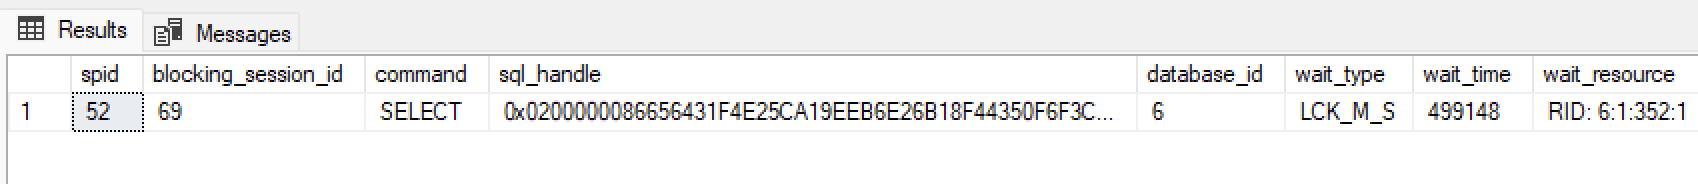
\includegraphics[width=\textwidth]{images/task-2/12.png}
  \caption{Результат выполнения запроса}
  \label{fig:task-2-12}
\end{figure}

С помощью кнопки <<\foreignlanguage{english}{Cancel Executing Query}>> на панели
инструментов (рисунок \ref{fig:task-2-13}), запрос, выполняемый во втором окне,
был отменен. После этого, с помощью инструкции <<\foreignlanguage{english}{SET
  LOCK\_TIMEOUT 5000}>> (рисунок \ref{fig:task-2-14}) было установлено время
ожидания блокировки в пять секунд. Как видно на рисунке \ref{fig:task-2-15},
после пяти секунд выполнение запроса завершилось с ошибкой.

\begin{figure}[H]
  \centering
  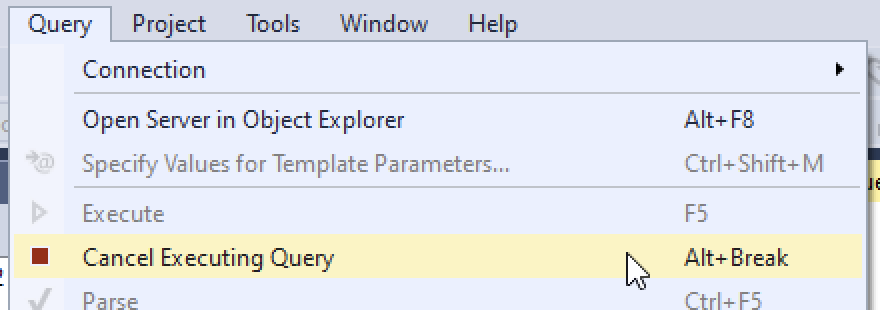
\includegraphics[width=0.7\textwidth]{images/task-2/13.png}
  \caption{Кнопка отмены выполнения запроса}
  \label{fig:task-2-13}
\end{figure}

\begin{figure}[H]
  \centering
  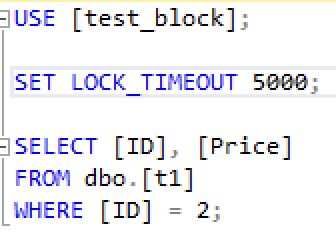
\includegraphics[width=0.4\textwidth]{images/task-2/14.png}
  \caption{Запрос с временем ожидания блокировки}
  \label{fig:task-2-14}
\end{figure}

\begin{figure}[H]
  \centering
  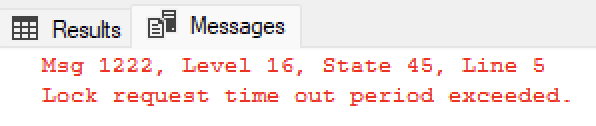
\includegraphics[width=0.5\textwidth]{images/task-2/15.png}
  \caption{Результат выполнения запроса}
  \label{fig:task-2-15}
\end{figure}

После этого, с помощью инструкции <<\foreignlanguage{english}{SET
  LOCK\_TIMEOUT -1}>> (рисунок \ref{fig:task-2-16}) время ожидание было возвращено
к значению по умолчанию. Затем, с помощью инструкции
<<\foreignlanguage{english}{KILL 69}>> (рисунок \ref{fig:task-2-17}) была
завершена транзакция, выполняемая в первом окне. После этого уже во втором окне
запрос был успешно выполнен, так как блокировка была снята (рисунок
\ref{fig:task-2-18}. Как видно, изменения из отменной транзакции не были
применены.

\begin{figure}[H]
  \centering
  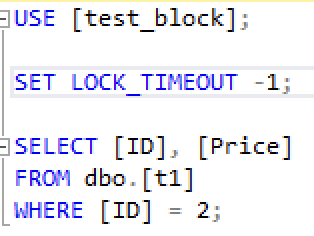
\includegraphics[width=0.4\textwidth]{images/task-2/16.png}
  \caption{Запрос с временем ожидания блокировки по умолчанию}
  \label{fig:task-2-16}
\end{figure}

\begin{figure}[H]
  \centering
  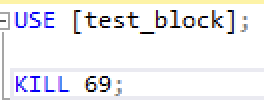
\includegraphics[width=0.4\textwidth]{images/task-2/17.png}
  \caption{Запрос для завершения транзакции в первом окне}
  \label{fig:task-2-17}
\end{figure}

\begin{figure}[H]
  \centering
  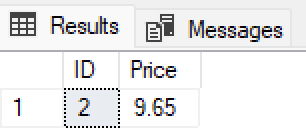
\includegraphics[width=0.4\textwidth]{images/task-2/18.png}
  \caption{Результат выполнения запроса во втором окне}
  \label{fig:task-2-18}
\end{figure}

\subsection{Третья задача}

\subsubsection{Уровень изоляции READ UNCOMMITTED}

Для выполнения данного задания было открыто два окна. В первом из них был
выполнен запрос, показанный на рисунке \ref{fig:task-3-1}. В нем создается
транзакция, изменяющая стоимость товара с идентификатором 2. При этом транзакция
не завершается. После выполнения данного запроса, как видно на рисунке
\ref{fig:task-3-2}, изменения были применены внутри транзакции.

\begin{figure}[H]
  \centering
  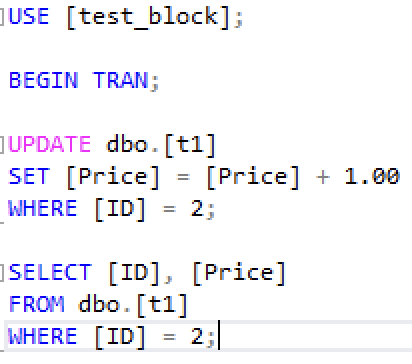
\includegraphics[width=0.6\textwidth]{images/task-3/1.png}
  \caption{Запрос с незавершенной транзакцией}
  \label{fig:task-3-1}
\end{figure}

\begin{figure}[H]
  \centering
  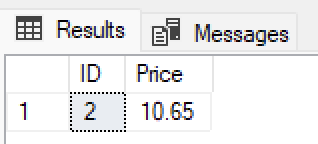
\includegraphics[width=0.5\textwidth]{images/task-3/2.png}
  \caption{Результат выполнения запроса}
  \label{fig:task-3-2}
\end{figure}

Запрос, приведенный на рисунке \ref{fig:task-3-3} сначала устанавливает уровень
изоляции <<\foreignlanguage{english}{READ UNCOMMITTED}>>, а затем читает
информацию о товаре из строки с идентификатором 2. Как видно на рисунке
\ref{fig:task-3-4}, блокировки в этом случае не произошло, при этом прочитанные
данные соответствует тем, что были получены в незавершенной транзакции.

\begin{figure}[H]
  \centering
  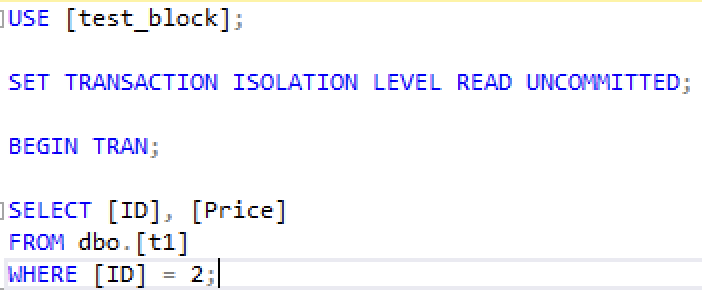
\includegraphics[width=0.7\textwidth]{images/task-3/3.png}
  \caption{
    Запрос с уровнем изоляции <<\foreignlanguage{english}{READ UNCOMMITTED}>>
  }
  \label{fig:task-3-3}
\end{figure}

\begin{figure}[H]
  \centering
  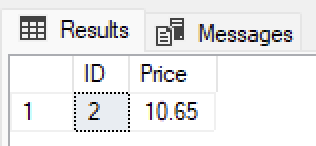
\includegraphics[width=0.5\textwidth]{images/task-3/4.png}
  \caption{Результат выполнения запроса}
  \label{fig:task-3-4}
\end{figure}

После этого в первом окне, с помощью запроса, показанного на рисунке
\ref{fig:task-3-5}, транзакция была отменена. Как видно на рисунке
\ref{fig:task-3-6}, изменения не были сохранены в базе данных.

\begin{figure}[H]
  \centering
  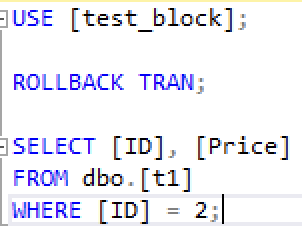
\includegraphics[width=0.5\textwidth]{images/task-3/5.png}
  \caption{Запрос для отмены транзакции}
  \label{fig:task-3-5}
\end{figure}

\begin{figure}[H]
  \centering
  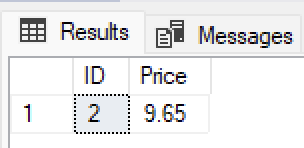
\includegraphics[width=0.5\textwidth]{images/task-3/6.png}
  \caption{Результат выполнения запроса}
  \label{fig:task-3-6}
\end{figure}

\subsubsection{Уровень изоляции READ COMMITTED}

В качестве примера в первом окне был использован тот же запрос, что показан на
рисунке \ref{fig:task-3-1}. После этого, во втором окне был выполнен запрос,
представленный на рисунке \ref{fig:task-3-7}. В данном запросе используется
уровень изоляции <<\foreignlanguage{english}{READ COMMITTED}>>. 

\begin{figure}[H]
  \centering
  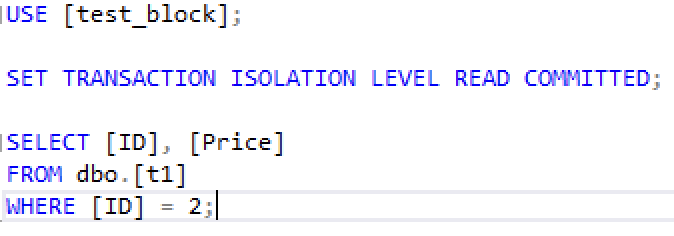
\includegraphics[width=0.8\textwidth]{images/task-3/7.png}
  \caption{
    Запрос с уровнем изоляции <<\foreignlanguage{english}{READ COMMITTED}>>
  }
  \label{fig:task-3-7}
\end{figure}

При выполнении данного запроса, так как желаемая строка была заблокирована,
запрос стал ожидать снятия блокировки. Для снятия блокировки использовался
запрос, показанный на рисунке \ref{fig:task-3-8}. В нем ранее выполненная
транзакция была отменена.

\begin{figure}[H]
  \centering
  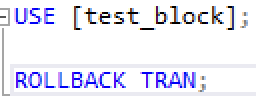
\includegraphics[width=0.4\textwidth]{images/task-3/8.png}
  \caption{Запрос с отменой транзакции}
  \label{fig:task-3-8}
\end{figure}

\subsubsection{Уровень изоляции REPEATABLE READ}

В первом окне был выполнен запрос, показанный на рисунке \ref{fig:task-3-9}. В
нем устанавливается уровень изоляции <<\foreignlanguage{english}{REPEATABLE
READ}>>, а также создается транзакция, в которой происходит считывание строки с
идентификатором 2. При этом транзакция не завершается. На рисунке
\ref{fig:task-3-10} приведен результат выполнения запроса.

\begin{figure}[H]
  \centering
  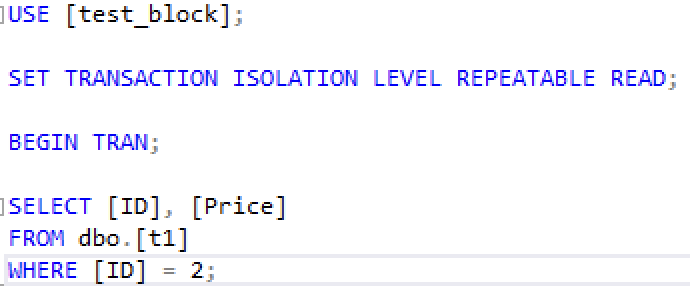
\includegraphics[width=0.8\textwidth]{images/task-3/9.png}
  \caption{
    Запрос с уровнем изоляции <<\foreignlanguage{english}{REPEATABLE READ}>>
  }
  \label{fig:task-3-9}
\end{figure}

\begin{figure}[H]
  \centering
  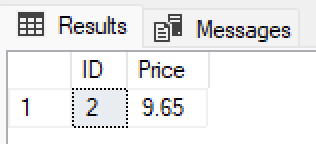
\includegraphics[width=0.4\textwidth]{images/task-3/10.png}
  \caption{Результат выполнения запроса}
  \label{fig:task-3-10}
\end{figure}

Во втором окне был выполнен запрос, приведенный на рисунке \ref{fig:task-3-11}.
В нем происходит попытка изменить строку также с идентификатором 2. Из-за
<<\foreignlanguage{english}{REPEATABLE READ}>> данный запрос не выполняется до
конца, а начинает ожидать завершения транзакции из первого окна.

\begin{figure}[H]
  \centering
  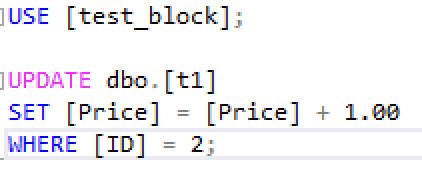
\includegraphics[width=0.5\textwidth]{images/task-3/11.png}
  \caption{Запрос с изменением заблокированной строки}
  \label{fig:task-3-11}
\end{figure}

На рисунке \ref{fig:task-3-12} приведен запрос, который завершает транзакцию в
первом окне. После выполнения данного запроса строка была разблокирована, а
потому запрос из второго окна был успешно выполнен (рисунок
\ref{fig:task-3-13}). Как видно на рисунке \ref{fig:task-3-14}, после выполнения
данного запроса цена была изменена.

\begin{figure}[H]
  \centering
  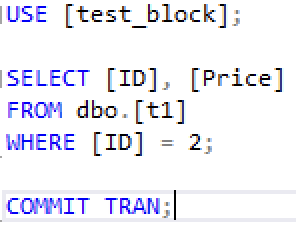
\includegraphics[width=0.4\textwidth]{images/task-3/12.png}
  \caption{Запрос с завершением транзакции}
  \label{fig:task-3-12}
\end{figure}

\begin{figure}[H]
  \centering
  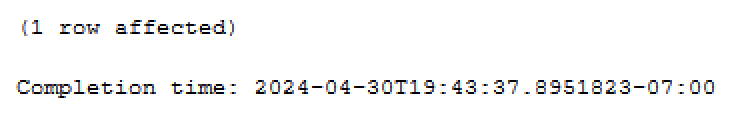
\includegraphics[width=0.8\textwidth]{images/task-3/13.png}
  \caption{Результат выполнения запроса из второго окна}
  \label{fig:task-3-13}
\end{figure}

\begin{figure}[H]
  \centering
  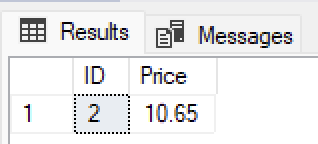
\includegraphics[width=0.4\textwidth]{images/task-3/14.png}
  \caption{Результат изменения цены}
  \label{fig:task-3-14}
\end{figure}

\subsubsection{Уровень изоляции SERIALIZABLE}

В первом окне был выполнен запрос, представленный на рисунке
\ref{fig:task-3-15}. В нем устанавливается уровень изоляции
<<\foreignlanguage{english}{SERIALIZABLE}>>, а также создается транзакция,
в которой считываются все строки со скидкой до 20\%. Результат выполнения
данного запроса представлен на рисунке \ref{fig:task-3-16}.

\begin{figure}[H]
  \centering
  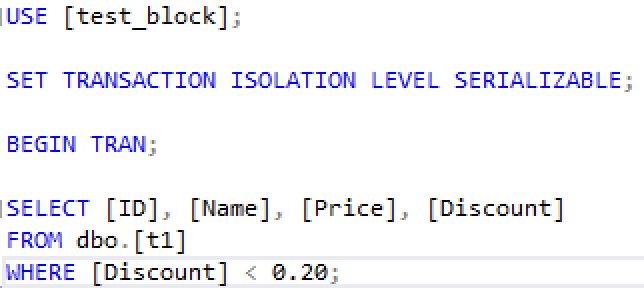
\includegraphics[width=0.6\textwidth]{images/task-3/15.png}
  \caption{
    Запрос с уровнем изоляции <<\foreignlanguage{english}{SERIALIZABLE}>>
  }
  \label{fig:task-3-15}
\end{figure}

\begin{figure}[H]
  \centering
  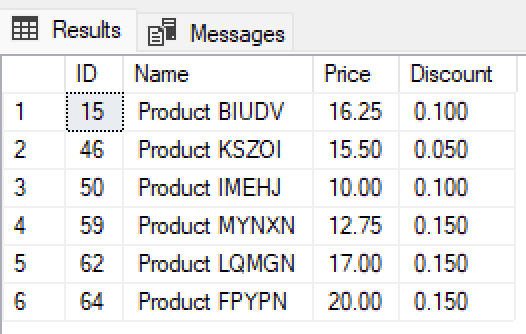
\includegraphics[width=0.6\textwidth]{images/task-3/16.png}
  \caption{Результат выполнения запроса}
  \label{fig:task-3-16}
\end{figure}

После этого во втором окне был выполнен запрос, показанный на рисунке
\ref{fig:task-3-17}. В нем происходит добавление нового товара со скидкой 5\%.
Однако, так как в предыдущем запросе был использован уровень изоляции
<<\foreignlanguage{english}{SERIALIZABLE}>>, данный запрос вынужден ожидать
окончание предыдущего запроса.

\begin{figure}[H]
  \centering
  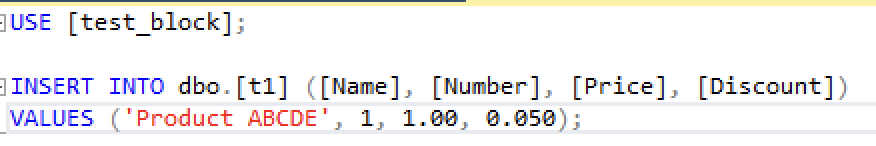
\includegraphics[width=0.7\textwidth]{images/task-3/17.png}
  \caption{Запрос с созданием нового товара}
  \label{fig:task-3-17}
\end{figure}

Затем в первом окне был выполнен запрос, представленный на рисунке
\ref{fig:task-3-18}. В нем происходит вывод всех товаров также со скидкой до
20\%, а затем завершение транзакции. Как видно на рисунке \ref{fig:task-3-19},
вывод идентичен тому, что был получен ранее. Новых товаров добавлено не было.

\begin{figure}[H]
  \centering
  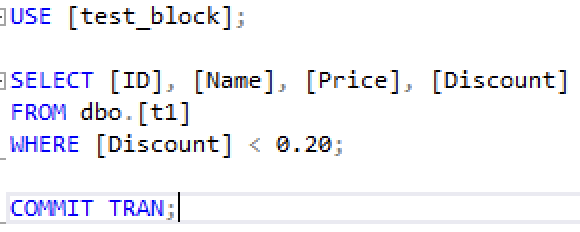
\includegraphics[width=0.6\textwidth]{images/task-3/18.png}
  \caption{Запрос с завершением транзакции}
  \label{fig:task-3-18}
\end{figure}

\begin{figure}[H]
  \centering
  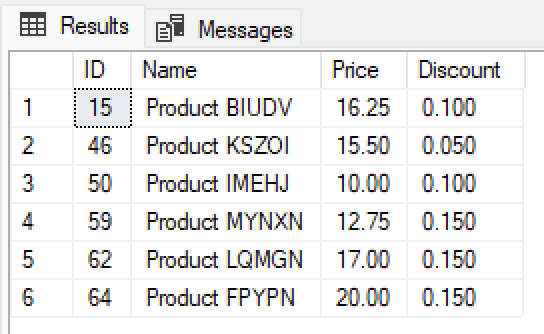
\includegraphics[width=0.6\textwidth]{images/task-3/19.png}
  \caption{Результат выполнения запроса}
  \label{fig:task-3-19}
\end{figure}

После выполнения запроса в первом окне, запрос во втором окне успешно
завершился. Это можно видеть на рисунке \ref{fig:task-3-20}.

\begin{figure}[H]
  \centering
  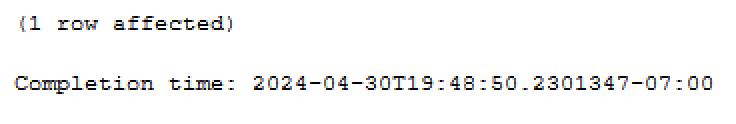
\includegraphics[width=0.8\textwidth]{images/task-3/20.png}
  \caption{Результат выполнения запроса во втором окне}
  \label{fig:task-3-20}
\end{figure}

В конце, для возврата уровня изоляции к значению, принятому по умолчанию, во
всех окнах был выполнен запрос, показанный на рисунке \ref{fig:task-3-21}.

\begin{figure}[H]
  \centering
  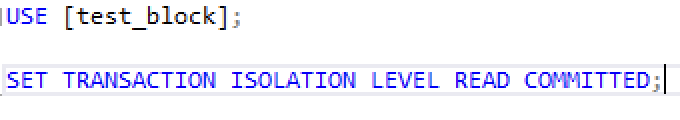
\includegraphics[width=0.8\textwidth]{images/task-3/21.png}
  \caption{Запрос для возврата уровня изоляции к значению по умолчанию}
  \label{fig:task-3-21}
\end{figure}

\section{Выводы и анализ результатов работы}

В данной лабораторной работе изучены способы работы с транзакциями и
блокировками в SSMS. При выполнении лабораторной работы были использованы
различные способы управления транзакциями. При создании транзакций были
рассмотрены различные виды блокировок: их различия, а также ситуации, когда
нужно использовать ту или иную блокировку. Как было показано, транзакции
являются очень удобным и необходимым инструментом при работе с СУБД. Без
транзакций работа с базой данных была бы куда сложнее и менее безопасной.

Цель, поставленная в начале работы, достигнута, задачи выполнены.

\end{document}
